
%(BEGIN_QUESTION)
% Copyright 2010, Tony R. Kuphaldt, released under the Creative Commons Attribution License (v 1.0)
% This means you may do almost anything with this work of mine, so long as you give me proper credit

The following PFD shows the ``loop'' for steam and water in a power boiler system, where fuel is burnt to produce electricity.  This particular power plant is located near the ocean, where saltwater is used to cool the steam turbine's exhaust back into water:

$$\includegraphics[width=15.5cm]{i03727x01.eps}$$

The purpose of the ``AAH'' instrument is to detect any leaks that might develop inside the condensor (heat exchanger).  What exactly is this analytical instrument measuring and what purpose does it serve in the context of the larger system?  What would be bad about having a small leak in the heat exchanger, anyway?

\vskip 20pt \vbox{\hrule \hbox{\strut \vrule{} {\bf Suggestions for Socratic discussion} \vrule} \hrule}

\begin{itemize}
\item{} Describe the difference between {\it saturated} steam and {\it superheated} steam. 
\item{} Would it be useful to place a conductivity sensor in either the saturated or superheated steam line?  Explain why or why not.
\item{} Would it be useful to place a conductivity sensor in the mud drum?  Explain why or why not.
\item{} One way to help avoid contamination due to leakage is to situate the heat exchanger with the proper pressure differential between the cooled and cooling fluids.  Describe how this ``pressure differential'' approach might be applied to this process, so that a heat exchanger leak would not be so disruptive to power plant operations.  Furthermore, identify where a differential pressure transmitter could be connected in this system to monitor the pressure difference.
\item{} Identify how the piping arrangement could be altered from what is shown in this diagram to help maintain a pressure differential between the tube and shell sides of the heat exchanger.
\item{} Examining this diagram, identify the purpose of the ``economizer'' in a boiler feedwater system.
\item{} Examining this diagram, describe the difference between ``saturated'' and ``superheated'' steam, and explain how both types of steam are produced.
\item{} Identify suitable level transmitter technologies for installation in the steam drum.
\item{} Identify suitable flowmeter technologies for installation in the feedwater line, and also the most desirable location(s).  Assume we need to know the {\it mass} flow rate for boiler feedwater, in units of pounds per minute.
\item{} Identify suitable flowmeter technologies for installation in the saturated steam line, and also the most desirable location(s).  Assume we need to know the {\it mass} flow rate for boiler steam output, in units of pounds per minute.
\item{} Identify suitable flowmeter technologies for installation in the burner's air line.
\item{} Identify suitable flowmeter technologies for installation in the burner's fuel line, assuming a liquid fuel.
\item{} Identify suitable flowmeter technologies for installation in the burner's fuel line, assuming a gaseous fuel.
\end{itemize}

\underbar{file i03727}
%(END_QUESTION)





%(BEGIN_ANSWER)


%(END_ANSWER)





%(BEGIN_NOTES)

The analytical alarm (AAH) in this system is a {\it conductivity} transmitter, measuring how electrically conductive the condensate is.  Boiler condensate is supposed to have minimal mineral content, and as such its conductivity should be really low.  If a leak develops in the heat exchanger, though, any intrusion of saltwater from the ocean will cause this conductivity to dramatically increase.

\vskip 10pt

A leak would be bad because minerals from the ocean water would begin to collect on the insides of the boiler tubes, choking them off and impeding heat transfer so that they would fail early.

%INDEX% Measurement, analytical: conductivity
%INDEX% Process: boiler condensate analysis

%(END_NOTES)

